\documentclass[11pt, fleqn]{article}

\usepackage{amsmath}
\usepackage{amsfonts}
\usepackage{amsthm}
\usepackage[margin=1in]{geometry} % To set the margin widths
\usepackage{graphicx}
%\usepackage{hyperref}
\usepackage{listings}
\usepackage{multirow}
\usepackage{tabularx}
\usepackage{varioref}
\usepackage{cleveref}  % this redefines vref to use cleverref
\usepackage{siunitx}
%\usepackage{subcaption}
\usepackage{subfig}
\usepackage{titlesec}
\usepackage{bm}

\crefname{equation}{equation}{equations}
\crefname{figure}{figure}{figures}

\sisetup{output-exponent-marker=\textsc{e}}

\titleformat{\section}[block]{\bfseries}{\thesection}{1em}{}


\setlength{\parskip}{12pt} % Sets a blank line in between paragraphs
\setlength\parindent{0pt} % Sets the indent for each paragraph to zero

\begin{document}

\title{Big Data: Homework 6}
\author{Will Clark \& Matthew DeLio \\ 41201-01}
\date{\today}
\maketitle

\section{K-Means Clustering} \label{sec:kmeans}

In this section, we cluster the 109th congress phrase-counts to see what information can be obtained.  To accomplish this, we employ the K-Means clustering algorithm.  To choose the ``optimal'' cluster size, we employed varied the cluster-size from 2 to 35 and then used BIC to select the K with the minimum BIC, which should, hopefully good OOS clustering abilities.  \Vref{fig:kmeans_ic_plot} shows a plot of the information criteria while varying K; while the BIC finds a minima at 15, the AICc never reaches a minima.

As discussed in class, these information criteria are of lower-quality than those used for regression.  A quick glance at \vref{tab:k_means_summary} backs up this theory as there are several clusters with just a single representative (leading us to believe that the cluster is overfitting), and no clear divide between the democrats, republicans, and independents.  A quick glance at the top-3 phrases used in each cluster is shown in \vref{tab:g_words}, shows that cluster phrases can be rather random.  Additionally, the bulk of the representatives are contained in a single cluster.  However, when the algorithm does have a clear separation between democrat and republican representatives, there is a clear divide.  Combining information from the cluster summary (\cref{tab:k_means_summary}) and the top-3 phrases table (\cref{tab:k_means_3}) phrases such as ``program.help'' vs ``illegal.immigration'' for Democrats and Republicans respectively indicate that the algorithm can cluster based on some partisan phrases.

As a final note, for an experiment to see if K-means would do a better job clustering the two parties, we ran k-means with a cluster-size of 2 \& 3.  In both instances (see \vref{tab:k_means_3} for K=3), the bulk of the representatives were clustered together as when K=15.  This begs the question: are the two parties really all that different after all?

\begin{figure}[!htb]
  \centering
  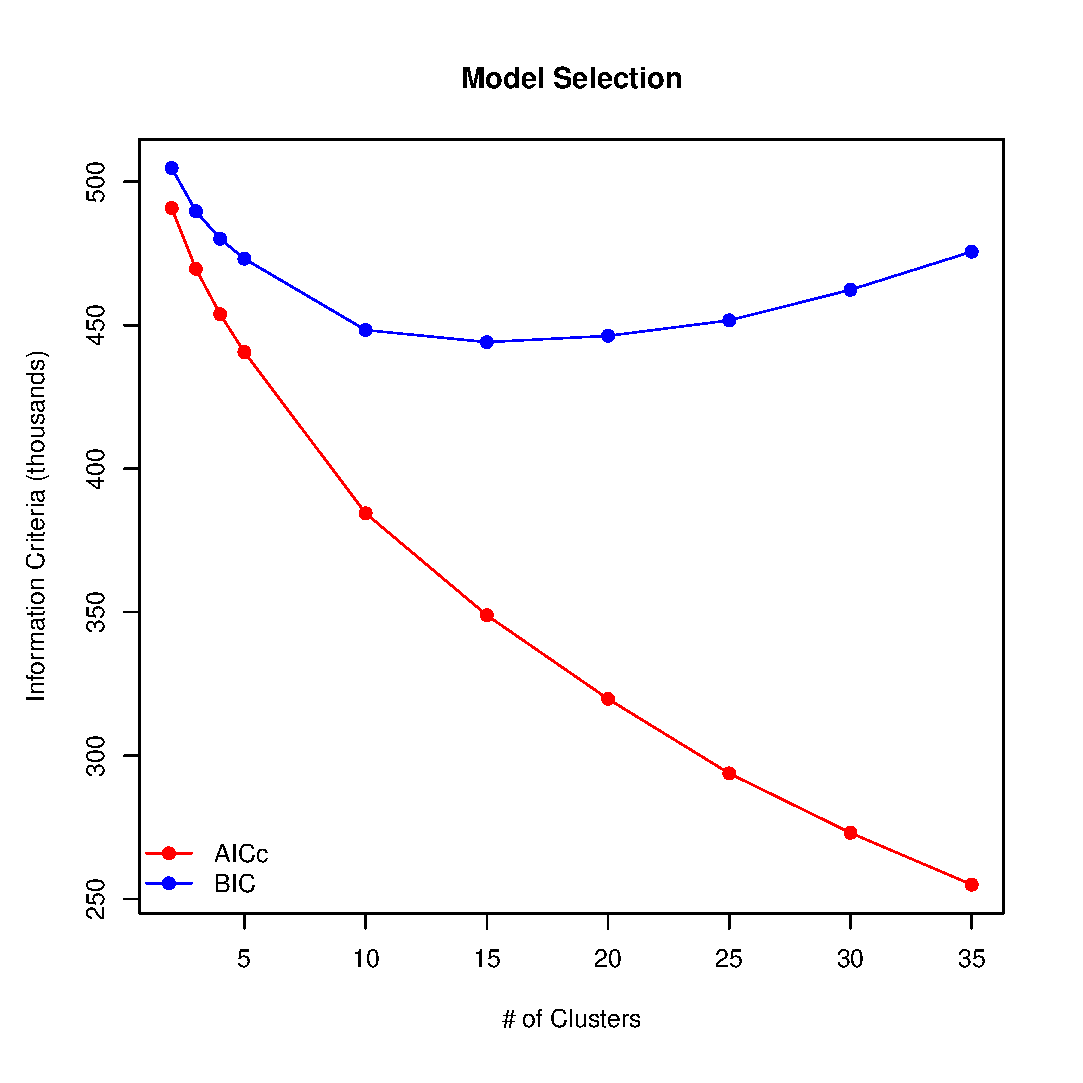
\includegraphics[scale=.5]{kmeans_ic_plot.eps}
  \caption{Informaton Criteria for Varying K-means}
  \label{fig:kmeans_ic_plot}
\end{figure}

% latex table generated in R 3.2.0 by xtable 1.7-4 package
% Fri May 22 07:11:07 2015
\begin{table}[ht]
\centering
\begin{tabular}{rlll}
  \hline
 & First & Second & Third \\ 
  \hline
1 & cut.funding & additional.funding & program.help \\ 
  2 & malpractice.insurance.rate & speaker.table & ending.september \\ 
  3 & buy.american.product & world.poorest.people & central.american.fre \\ 
  4 & boy.girl.club & republican.senator & check.bal \\ 
  5 & outing.cia.agent & cia.agent & social.security.plan \\ 
  6 & final.minute & legislative.session & date.time \\ 
  7 & summa.cum.laude & justice.priscilla.owen & supreme.court.united \\ 
  8 & committe.commerce.science & global.war & illegal.immigration \\ 
  9 & international.labor.organization & medic.leave.act & funding.cut \\ 
  10 & northern.ireland & children.live.poverty & increase.minimum.wage \\ 
  11 & low.income.individual & tax.relief.package & increase.taxe \\ 
  12 & tax.cut.spending & additional.tax.cut & record.deficit \\ 
  13 & fuel.efficiency & invasion.iraq & bankruptcy.court \\ 
  14 & arab.oil.embargo & pluripotent.stem.cel & percent.growth.rate \\ 
  15 & violent.sexual.predator & sole.source.contract & integrated.oil.compani \\ 
   \hline
\end{tabular}
\caption{Top Phrases by Cluster} 
\label{tab:g_words}
\end{table}


\section{Topic Model}

A topic model was constructed using \texttt{topics} command in R.  This multinomial model clusters the phrases used by the representatives into topics and is supposed to do a much better job than the K-means cluster from earlier.  The top-3 phrases for each topic (sorted by largest $P(phrase_i|topic_k)$) are found in \vref{tab:tpcs3}.  These phrases do indicate that this method does a really good job of finding related phrases.  There are few clusters that should probably be merged or otherwise modified (namely the 9th and 10th topics).  However, the vast majority of topics contain phrases that are very much inter-related; they are, in fact topics.  For example, the first topic appears to be about immigration, the second about civil rights, etc.

% latex table generated in R 3.2.0 by xtable 1.7-4 package
% Fri May 22 07:11:36 2015
\begin{table}[ht]
\centering
\begin{tabular}{rlll}
  \hline
 & First & Second & Third \\ 
  \hline
1 & private.property & illegal.alien & illegal.immigration \\ 
  2 & african.american & civil.right & head.start \\ 
  3 & american.people & private.account & veteran.health \\ 
  4 & tax.relief & american.people & death.tax \\ 
  5 & american.people & iraqi.people & saddam.hussein \\ 
  6 & appropriation.bil & natural.ga & climate.change \\ 
  7 & postal.service & endangered.speci.act & strong.support \\ 
  8 & class.action & american.people & chief.justice \\ 
  9 & oil.compani & prescription.drug & foreign.oil \\ 
  10 & stem.cel & natural.ga & cel.research \\ 
  11 & minimum.wage & credit.card & low.income \\ 
  12 & trade.agreement & fre.trade & central.american \\ 
  13 & domestic.violence & hate.crime & violence.women \\ 
   \hline
\end{tabular}
\caption{Top-3 Topic Phrases} 
\label{tab:tpcs3}
\end{table}


\section{Connecting Unsupervised Clusters to Partisanship}
\subsection{Party Membership by K-means Cluster}
See \vref{tab:k_means_summary} for the party membership by K-means cluster.  As mentioned in the \cref{sec:kmeans}, the K-means clustering does not yield a ton of useful information about a representatives affiliation.  There are a handful of senators and congressman that are clearly grouped into their party, however, the vast majority end up in a single cluster.  This is likely because they argue against each other and therefore use each others' words in their speeches.  However, if taken at face-value, the cluster with almost an equal amount of republican and democratic members would likely denote phrases that are considered non-partisan.  These ``non-partisan'' phrases are found in \vref{tab:k_means_nonpart}, and do actually tend to indicate non-partisan phrases.

% latex table generated in R 3.2.0 by xtable 1.7-4 package
% Fri May 22 07:11:36 2015
\begin{table}[ht]
\centering
\begin{tabular}{rrrrrr}
  \hline
 & \# Dem & \# Ind & \# Rep & Total & mean(RepShare) \\ 
  \hline
1 &  40 &   1 &   0 &  41 & 0.42 \\ 
  2 & 185 &   1 & 238 & 424 & 0.51 \\ 
  3 &   1 &   0 &   0 &   1 & 0.44 \\ 
  4 &   1 &   0 &   0 &   1 & 0.40 \\ 
  5 &   2 &   0 &   0 &   2 & 0.27 \\ 
  6 &   0 &   0 &   1 &   1 & 0.57 \\ 
  7 &   0 &   0 &   6 &   6 & 0.61 \\ 
  8 &   0 &   0 &  37 &  37 & 0.59 \\ 
  9 &   8 &   0 &   0 &   8 & 0.43 \\ 
  10 &   1 &   0 &   0 &   1 & 0.37 \\ 
  11 &   0 &   0 &   2 &   2 & 0.50 \\ 
  12 &   2 &   0 &   0 &   2 & 0.61 \\ 
  13 &   1 &   0 &   0 &   1 & 0.45 \\ 
  14 &   0 &   0 &   1 &   1 & 0.65 \\ 
  15 &   1 &   0 &   0 &   1 & 0.64 \\ 
   \hline
\end{tabular}
\caption{Cluster Summary for k=15 (min BIC)} 
\label{tab:k_means_summary}
\end{table}

% latex table generated in R 3.1.2 by xtable 1.7-4 package
% Fri May 22 01:26:24 2015
\begin{table}[ht]
\centering
\begin{tabular}{rr}
  \hline
 & Relative Frequency \\ 
  \hline
malpractice.insurance.rate & 0.02 \\ 
  speaker.table & 0.02 \\ 
  ending.september & 0.02 \\ 
  national.homeownership.month & 0.02 \\ 
  united.postal.service & 0.01 \\ 
  columbia.river.gorge & 0.01 \\ 
  national.heritage.corridor & 0.01 \\ 
  commonly.prescribed.drug & 0.01 \\ 
  wild.bird & 0.01 \\ 
  driver.education & 0.01 \\ 
   \hline
\end{tabular}
\caption{Top 10 Non-Partisan Phrases from K-means} 
\label{tab:k_means_nonpart}
\end{table}


\subsection{Non-Partisan Topics}

Here we plot the topic-frequencies based on party affiliation.  \Vref{fig:topic} clearly shows that some topics are much more partisan than others.  For the topics with large deviation between the two parties, we can (using \vref{tab:tpcs3}) see that some topics, such as illegal immigration and civil rights, tend to align with our intuition on which phrases would be used more often by party members.  For the most part, these differences in frequencies exist and are quite noticeable.  However, one of the topics (\#7) appears to be non-partisan.  \Vref{tab:non_part_topics} shows the top 10 phrases from that topic and intuition confirms that many of these phrases are fairly non-partisan.

\begin{figure}[!htb]
  \centering
  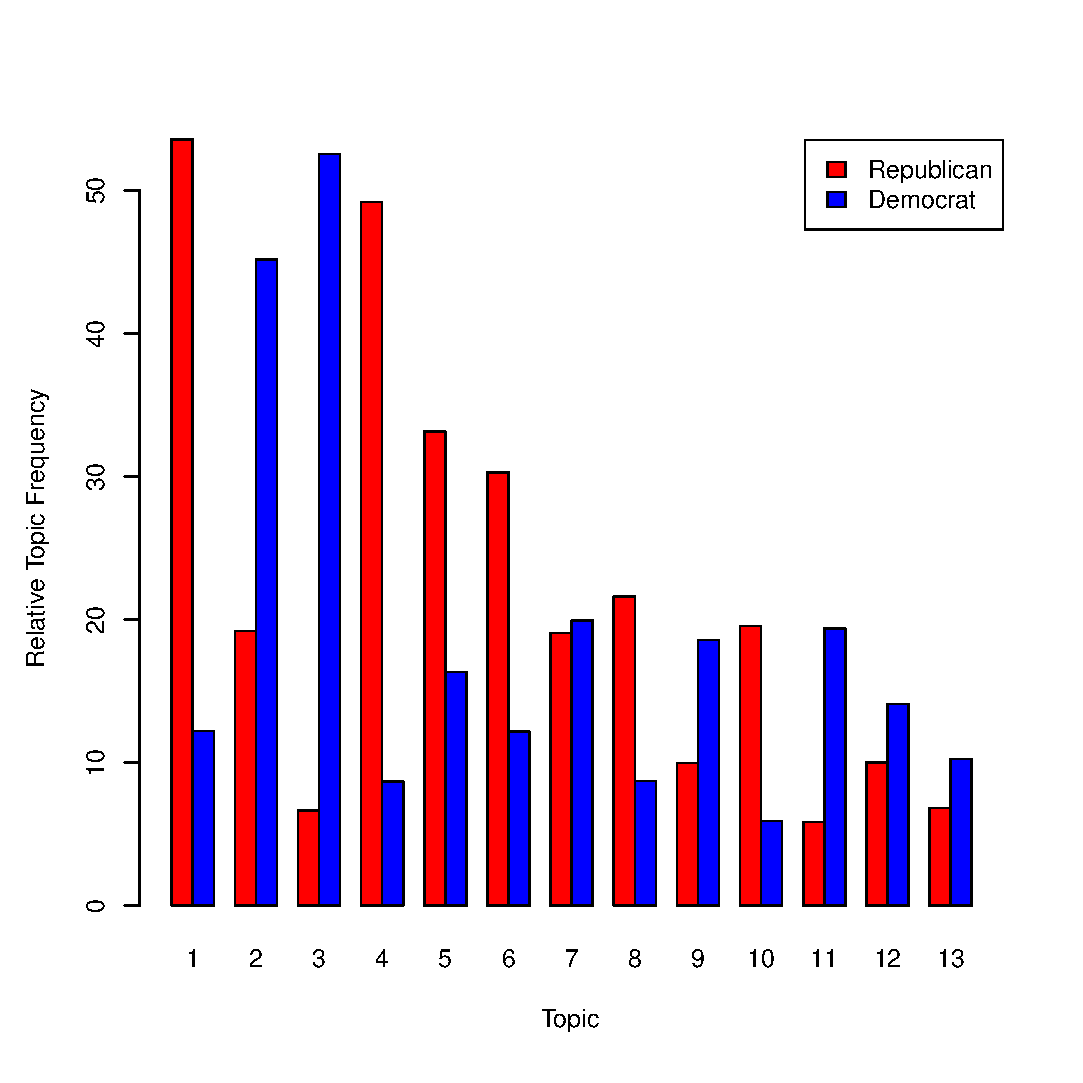
\includegraphics[scale=.5]{topic.eps}
  \caption{Partisan Topic Frequencies}
  \label{fig:topic}
\end{figure}

% latex table generated in R 3.1.2 by xtable 1.7-4 package
% Fri May 22 02:15:27 2015
\begin{table}[ht]
\centering
\begin{tabular}{rr}
  \hline
 & $\theta$ \\ 
  \hline
postal.service & 0.080 \\ 
  strong.support & 0.030 \\ 
  post.office & 0.029 \\ 
  endangered.speci.act & 0.029 \\ 
  passenger.rail & 0.028 \\ 
  drinking.water & 0.026 \\ 
  estate.tax & 0.024 \\ 
  appropriation.bil & 0.018 \\ 
  enemy.combatant & 0.018 \\ 
  water.act & 0.016 \\ 
   \hline
\end{tabular}
\caption{Non-Partisan Topic Words} 
\label{tab:non_part_topics}
\end{table}


\subsection{Party Membership/Share by Topic}

In this section, we use the results from the topic clustering to predict party membership.  We employ a gamma lasso with and without cross-validation to regress political affiliation onto the topic $\omega$'s chosen for each representative.  In general $\omega$'s give the percentage of a document (in this case a collection of speeches by a representative) that belongs to a given topic.  The hope is that the topics that are more likely to be discussed by, say a democrat, would help predict their party affiliation.  The gamma lasso and the cross-validated gamma lasso both include all 13 topics in the model, but completely disagree on the values of the information criteria (likely due to the small number of degrees of freedom).  \Vref{tab:topic_rep} shows that all three of the information criteria choose all 13 covariates and provide an in-sample $R^2$ of 56\%.  The OOS $R^2$ for the model chosen by cv.gamlr (using the CV.min rule) is a bit lower at $R^2=52\%$.

% latex table generated in R 3.2.0 by xtable 1.7-4 package
% Fri May 22 07:11:36 2015
\begin{table}[ht]
\centering
\begin{tabular}{rrrr}
  \hline
 & $\log(\lambda)$ & $R^2$ & Covariates Selected \\ 
  \hline
AICc & -7.86 & 0.56 &  13 \\ 
  AIC & -7.86 & 0.56 &  13 \\ 
  BIC & -7.86 & 0.56 &  13 \\ 
  CV.Min & -5.88 & 0.53 &  13 \\ 
  CV.1se & -3.97 & 0.50 &  13 \\ 
   \hline
\end{tabular}
\caption{ICs for Republican $\sim$ Topic $\omega$} 
\label{tab:topic_rep}
\end{table}


Here we regress the ``republican share'' onto our topics.  While very similar to regressing the party membership above, this measure allows us to determine how much a the use of certain topics will predict how large the republican share is in one's district.  Note, that this might not predict who is a democrat vs a republican; in fact, we would expect that in contested districts/states, the republican share to be quite large even if the sitting representative is a democrat.  As before the gamma lasso with/without cross-validation is performed; the results are shown in \vref{tab:topic_repshare}.  Again we see that the in-sample $R^2$ each of the ICs is 37\%.  Using cross-validation and the CV.min selection rule, this $R^2$ drops to 35\%; just a touch lower than the in-sample ones.

% latex table generated in R 3.2.0 by xtable 1.7-4 package
% Fri May 22 07:11:37 2015
\begin{table}[ht]
\centering
\begin{tabular}{rrrr}
  \hline
 & $\log(\lambda)$ & $R^2$ & Covariates Selected \\ 
  \hline
AICc & -7.50 & 0.38 &  14 \\ 
  AIC & -7.50 & 0.38 &  14 \\ 
  BIC & -5.73 & 0.37 &  12 \\ 
  CV.Min & -7.50 & 0.34 &  14 \\ 
  CV.1se & -4.75 & 0.31 &  11 \\ 
   \hline
\end{tabular}
\caption{ICs for Republican Share $\sim$ Topic $\omega$} 
\label{tab:topic_repshare}
\end{table}


Finally, we regress the party affiliation and republican share (separately) onto phrase frequency (measured in \%).  From \vref{tab:repx,tab:repsharex}, we see that, in both cases, AICc and CV.Min disagree quite a bit on the number of covariates to include.  Also, in-sample predictive power for the republican share (using AICc) is much higher than the out-of-sample one predicted/measured by the cross-validated gamma lasso.  Similarly, the $\lambda$ and $R^2$ found using AICc and CV.Min for the party affiliation also disagree widely.  This tends to indicate the phrase percentage, is not a great predictor of either of these. 

% latex table generated in R 3.1.2 by xtable 1.7-4 package
% Fri May 22 03:00:40 2015
\begin{table}[ht]
\centering
\begin{tabular}{rrrr}
  \hline
 & $\log(\lambda)$ & $R^2$ & Covariates Selected \\ 
  \hline
AICc & -2.78 & 0.24 &  32 \\ 
  AIC & -6.04 & 0.96 & 241 \\ 
  BIC & -2.27 & 0.08 &   6 \\ 
  CV.Min & -4.08 & 0.37 & 188 \\ 
  CV.1se & -3.20 & 0.29 &  92 \\ 
   \hline
\end{tabular}
\caption{ICs for Republican $\sim$ Phrase \%} 
\label{tab:repx}
\end{table}

% latex table generated in R 3.1.2 by xtable 1.7-4 package
% Fri May 22 03:01:27 2015
\begin{table}[ht]
\centering
\begin{tabular}{rrrr}
  \hline
 & $\log(\lambda)$ & $R^2$ & Covariates Selected \\ 
  \hline
AICc & -4.83 & 0.62 & 112 \\ 
  AIC & -7.80 & 0.98 & 473 \\ 
  BIC & -3.71 & 0.12 &   6 \\ 
  CV.Min & -4.22 & 0.19 &  51 \\ 
  CV.1se & -3.94 & 0.13 &  19 \\ 
   \hline
\end{tabular}
\caption{ICs for Republican Share $\sim$ Phrase \%} 
\label{tab:repsharex}
\end{table}


\Vref{tab:repx_coef_p,tab:repx_coef_n} show both the positive and negative the phrase percentage coefficients that predict the odds of a representative being a republican.  The signals selected are actually, intuitively quite good; however, there are not too many signals actually selected in the end (only 4 signals that increase the odds of a republican and 32 that decrease).  The model is perhaps underfit by the AICc, but, ultimately, by not distilling the phrases into a more usable form, the signals, by themselves are just not that strong.  In this sense, the distillation of the phrases into topics gives us a powerful tool to analyze data.

% latex table generated in R 3.2.0 by xtable 1.7-4 package
% Fri May 22 07:11:38 2015
\begin{table}[ht]
\centering
\begin{tabular}{rr}
  \hline
 & Coef \\ 
  \hline
global.war & 0.0299 \\ 
  oil.food & 0.0191 \\ 
  driver.license & 0.0042 \\ 
  death.tax & 0.0038 \\ 
   \hline
\end{tabular}
\caption{Top Phrases that Increase Odds of Predicting Republican} 
\label{tab:repx_coef_p}
\end{table}

% latex table generated in R 3.1.2 by xtable 1.7-4 package
% Fri May 22 03:22:09 2015
\begin{table}[ht]
\centering
\begin{tabular}{rr}
  \hline
 & Coef \\ 
  \hline
budget.cut & -0.6597 \\ 
  tax.cut.wealthy & -0.5788 \\ 
  live.poverty & -0.4954 \\ 
  privatize.social.security & -0.4033 \\ 
  cost.war & -0.3930 \\ 
   \hline
\end{tabular}
\caption{Top Phrases that Decrease Odds of Predicting Republican} 
\label{tab:repx_coef_n}
\end{table}



\clearpage
\section{Appendix}

% latex table generated in R 3.1.2 by xtable 1.7-4 package
% Fri May 22 00:23:56 2015
\begin{table}[ht]
\centering
\begin{tabular}{rrrrrr}
  \hline
 & \# Dem & \# Ind & \# Rep & Total & mean(RepShare) \\ 
  \hline
1 &   2 &   0 &   0 &   2 & 0.41 \\ 
  2 &  34 &   0 &   9 &  43 & 0.47 \\ 
  3 & 206 &   2 & 276 & 484 & 0.52 \\ 
   \hline
\end{tabular}
\caption{Cluster Summary for K=3} 
\label{tab:k_means_3}
\end{table}


\begin{figure}
  \centering
  \begin{subfigure}[b]{0.49\textwidth}
    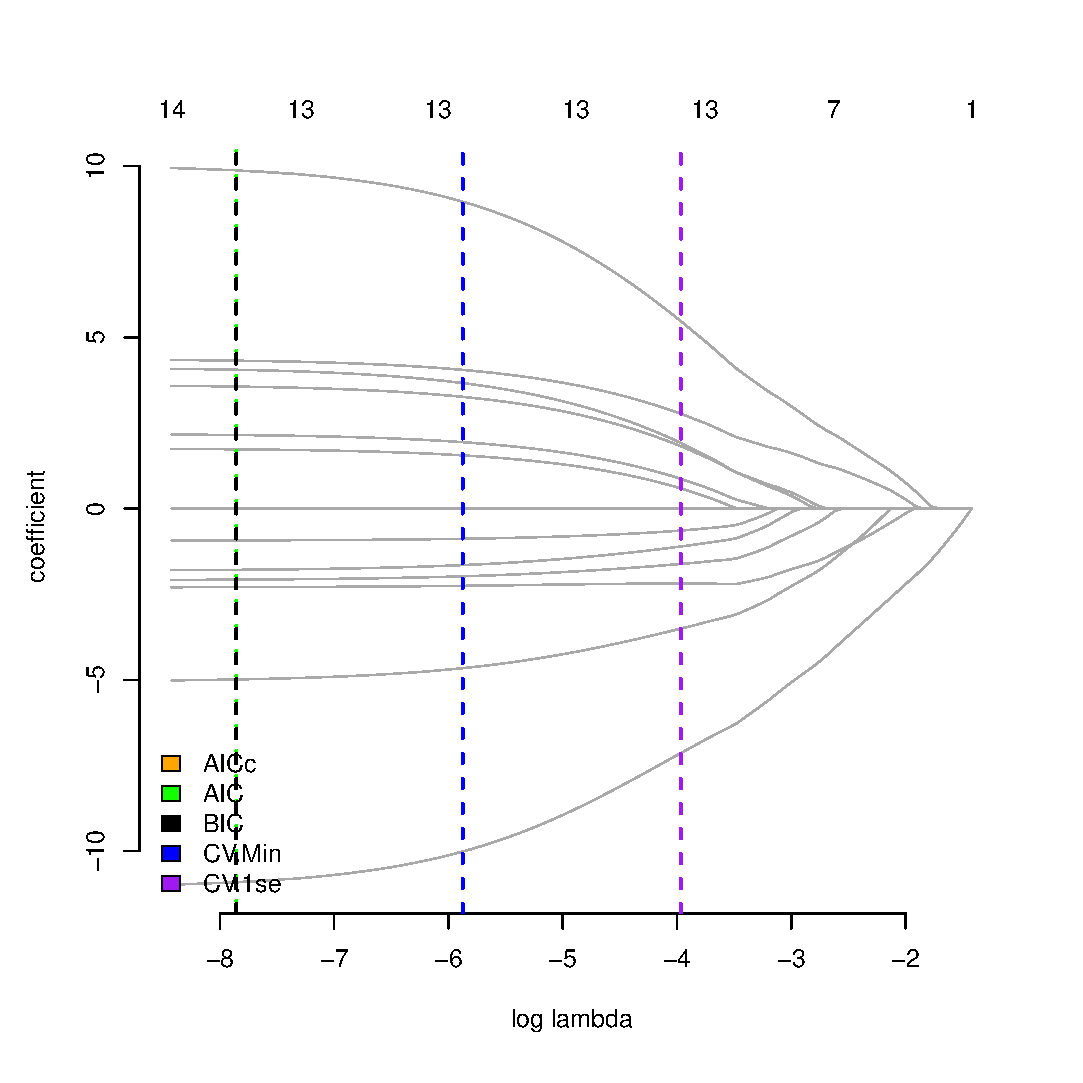
\includegraphics[width=\textwidth]{tpcs_rep.eps}
    \caption{Regressing Party Affiliation}
    \label{fig:tpcs_rep}
  \end{subfigure}
  \hfill
  \begin{subfigure}[b]{0.49\textwidth}
    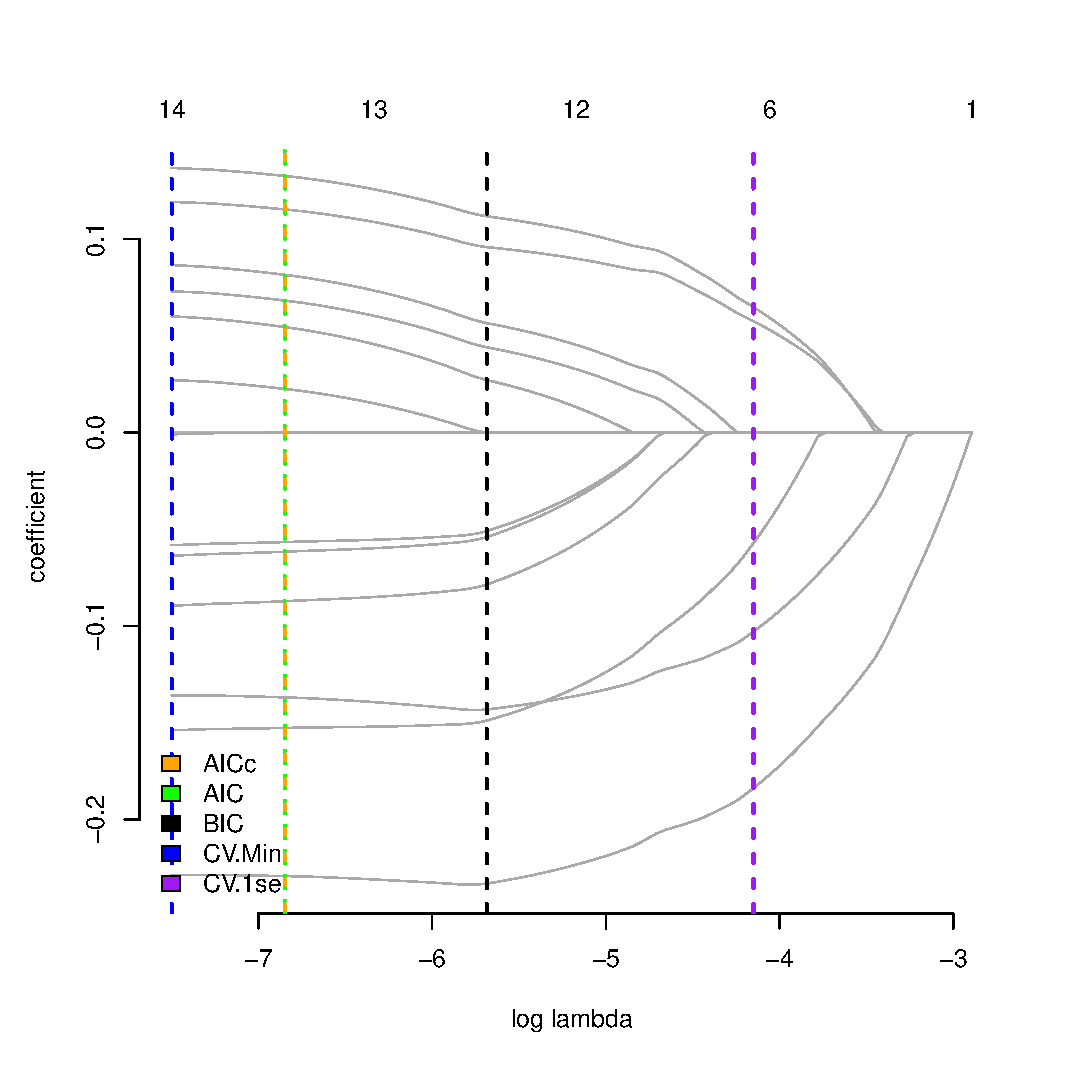
\includegraphics[width=\textwidth]{tpcs_rep_share.eps}
    \caption{Regressing District Republican Share}
    \label{fig:tpcs_repshare}
  \end{subfigure}
  \caption{Topics as Predictors}
\end{figure}

\begin{figure}
  \centering
  \begin{subfigure}[b]{0.49\textwidth}
    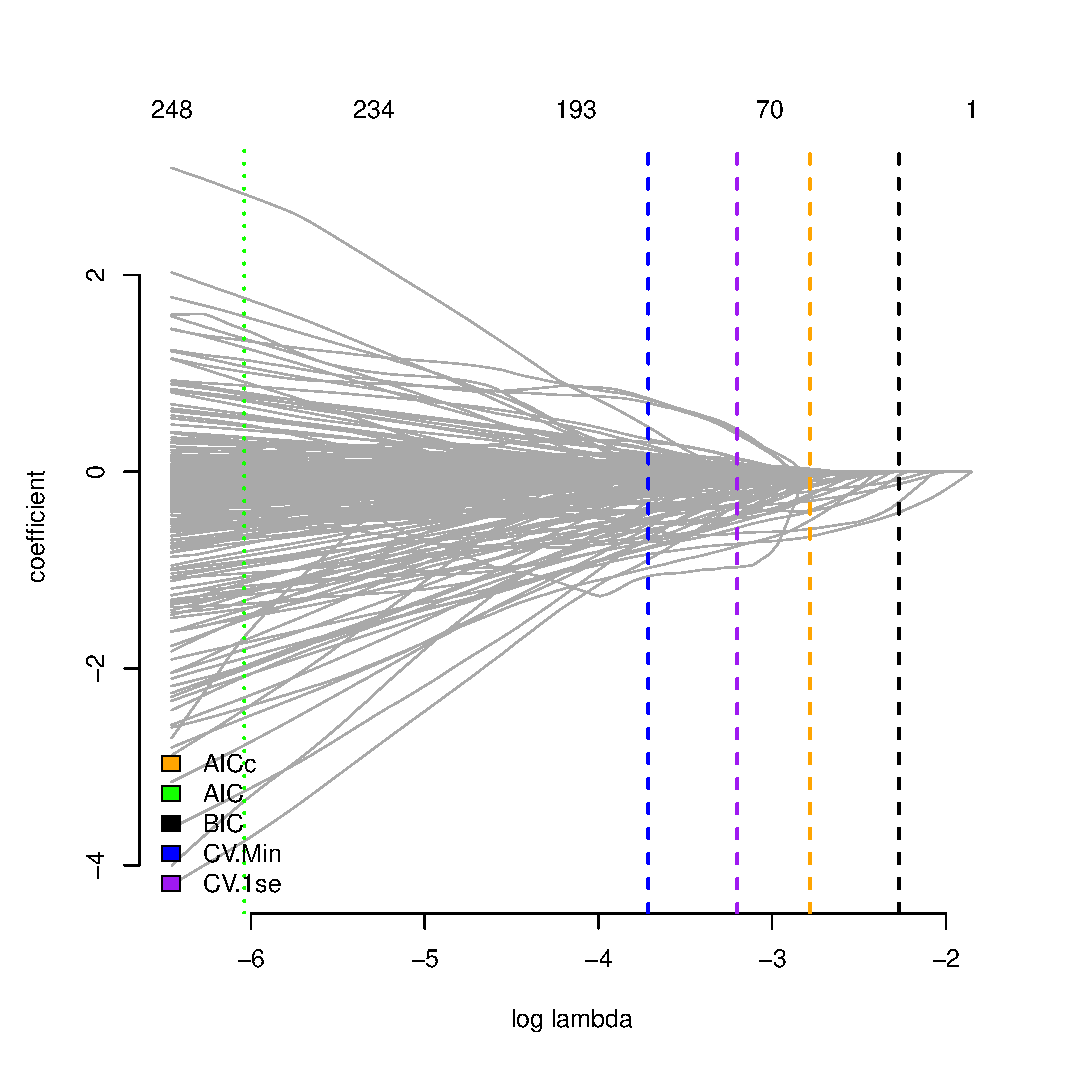
\includegraphics[width=\textwidth]{reg_phrase_pcnt.eps}
    \caption{Regressing Party Affiliation}
    \label{fig:pcnt_rep}
  \end{subfigure}
  \hfill
  \begin{subfigure}[b]{0.49\textwidth}
    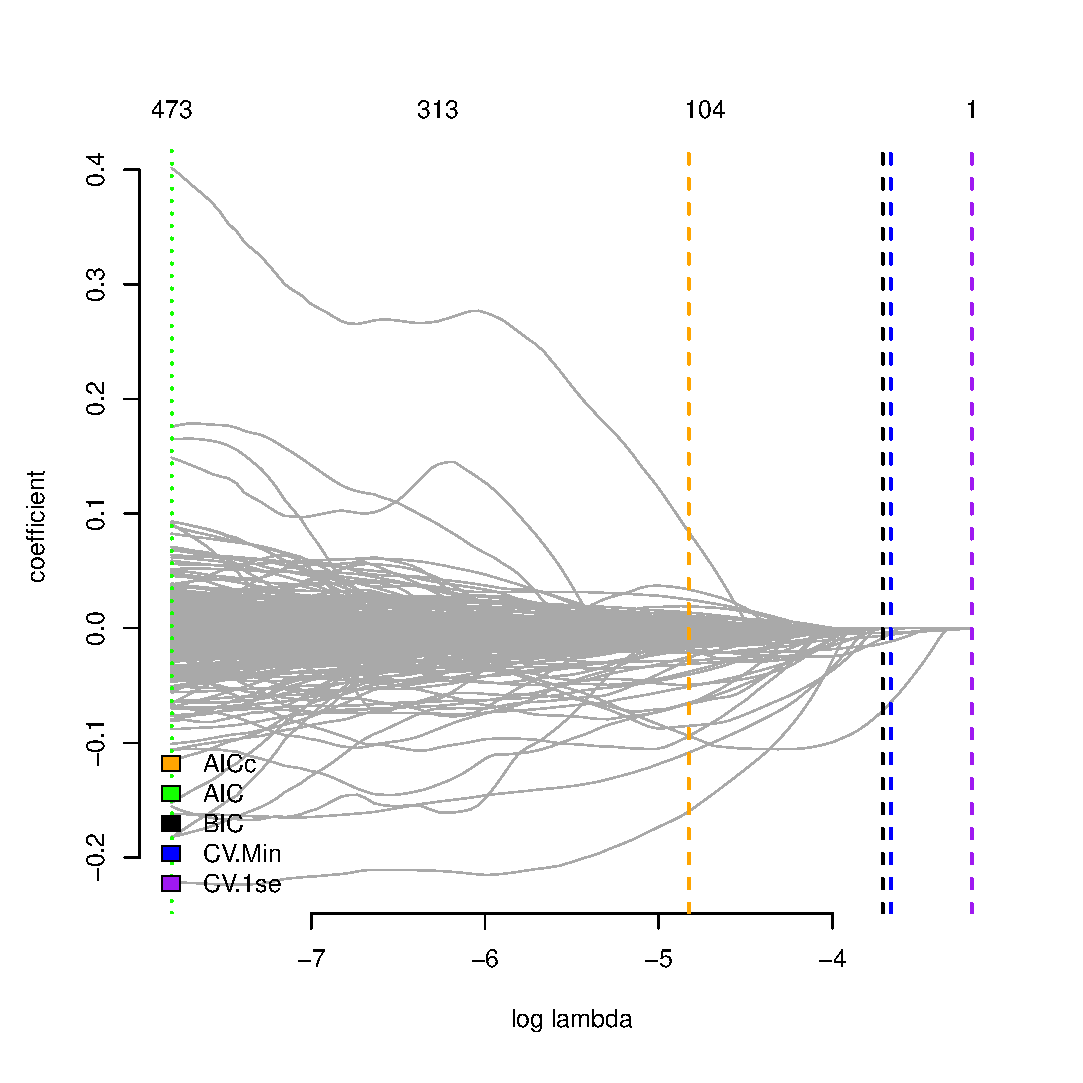
\includegraphics[width=\textwidth]{reg_phrase_pcnt_repshare.eps}
    \caption{Regressing District Republican Share}
    \label{fig:pcnt_rep_share}
  \end{subfigure}
  \caption{Phrase \% as Predictors}
\end{figure}


% \input{.tex}

% \begin{figure}
%   \centering
%   \begin{subfigure}[b]{0.49\textwidth}
%     \includegraphics[width=\textwidth]{.eps}
%     \caption{}
%     \label{fig:}
%   \end{subfigure}
%   \hfill
%   \begin{subfigure}[b]{0.49\textwidth}
%     \includegraphics[width=\textwidth]{.eps}
%     \caption{}
%     \label{fig:}
%   \end{subfigure}
%   \caption{}
% \end{figure}

% \begin{figure}[!htb]
%   \centering
%   \includegraphics[scale=.5]{.eps}
%   \caption{}
%   \label{fig:}
% \end{figure}

\end{document}